\section{Introduction} \label{chap:Introduction}
    % IQP Paper Guidelines 
    % https://www.wpi.edu/sites/default/files/IQP_Writing_Guidelines.pdf

    % QRP Paper
    % https://web.wpi.edu/Pubs/E-project/Available/E-project-042518-003336/unrestricted/QRP_FinalReport.pdf
    %Robodog
    %https://web.wpi.edu/Pubs/E-project/Available/E-project-042717-152039/unrestricted/MQP_RoboDog_Final_Report.pdf

    The field of quadrped robotics, or the study of 4-legged robots, has been inspired by the limitation of wheeled and tracked robotic systems. These systems favor flat terrain and struggle with extremely rough, uneven or rocky terrain. On the other hand, quadrupedal systems excel in these environments. When it comes to traversing complex terrains climbing up obstacles such as stairs and rocky mountain sides there are no better systems than legged ones. Quadruped systems have huge potential because of their ability to navigate these nonuniform surfaces make them ideal for exploration or providing assistance in the average home, where there may be unexpected obstacles to climb over. Using quadrupeds to explore locations wheeled robots can't is not just important here on earth but would also open a world of opportunities on other planets or moons in our strive for space exploration. In the home, quadrupeds can be used to navigate stairs or obstacles on the ground. They would allow us to create robotic assistants without having to restructure our homes or workplaces to accommodate a wheeled robot. Additionally they have many applications in the military as well. These kinds of robots are already being designed for reconnaissance or search and rescue and the United States military has contracted several of these robots to be used as robotic mules that can carry heavy items or people through the rough battlefield terrain. Since quadrupedal robots are relatively compelx to manufacture, due to their abundance of components and many moving parts, the industry as a whole has had difficulty expanding. Currently, the only way to learn, experiment, deveop, or create capable quadruped robots is to have the prowness of companies like DARPA (Defense Advanced Research Projects Agency) or Boston Dynamics. However, with new inexpensive processing technology and better manufacturing technologies like 3D printing, quadrupeds are on the brink of becoming more affordable than ever, allowing students and other robotics enthusiasts to explore the realm of quadrupedal systems.
    
    \begin{figure}
        \centering
        \parbox{0.7\linewidth}{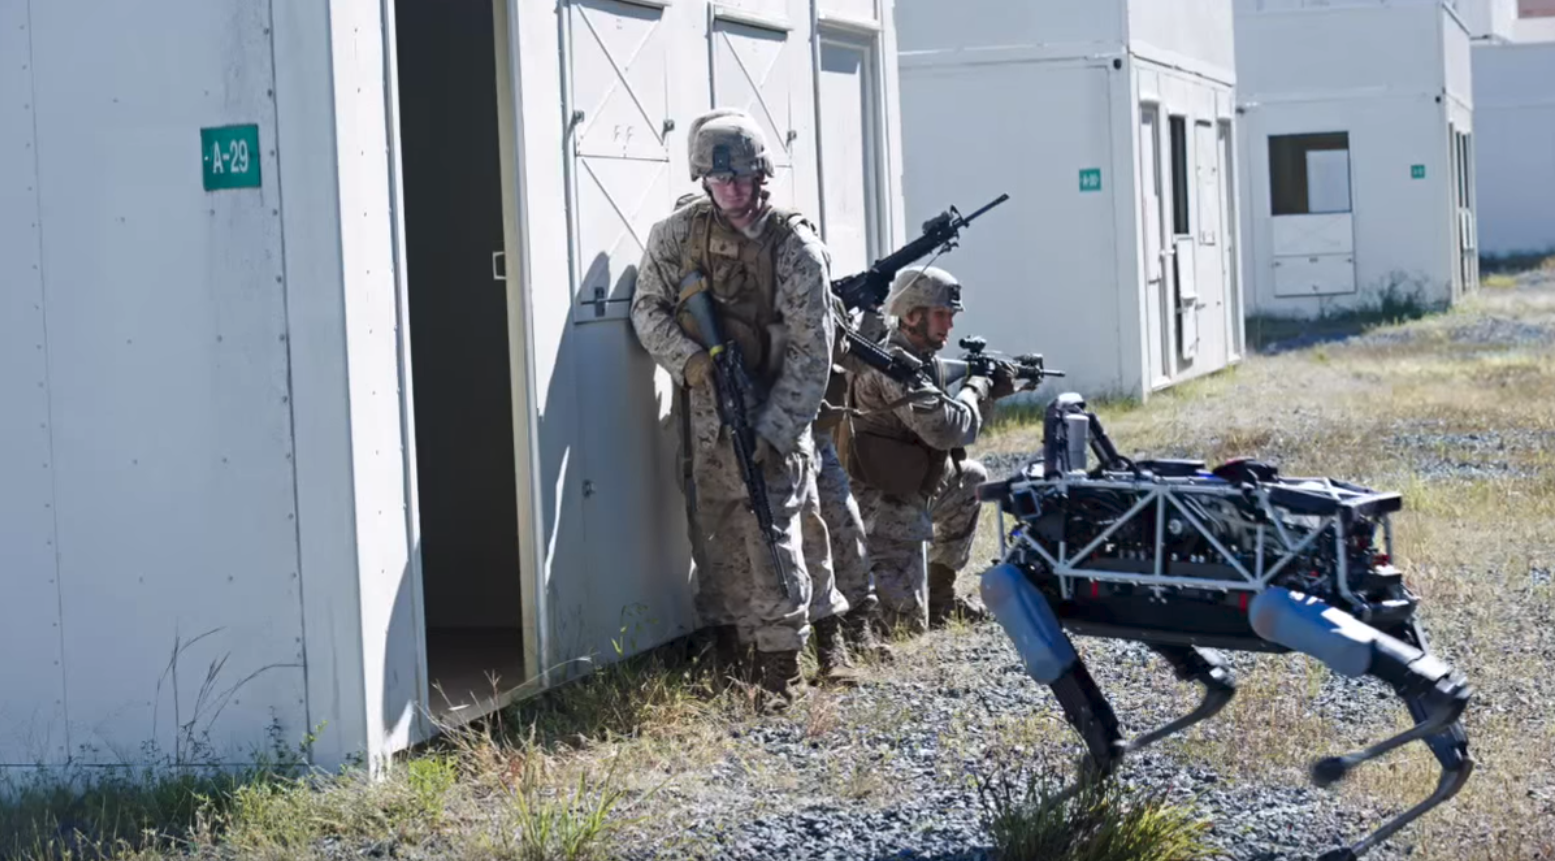
\includegraphics[width=0.7\textwidth]{figures/BostonDynamicsSpotMilitary.png}}
        \caption{Boston Dynamics' Spot during Military Trials with the Department of Defense}
        \label{fig:SpotMilitary} 
    \end{figure}
    
    % Add QRP cite, not working for some reason
    In the past few years, several MQPs have been attempted to design and build a walking quadruped for research purposes. Before beginning this project we looked into past work from the Quadruped Research Project (QRP) MQP, the RoboDog MQP,\cite{RoboDog_MQP} and the HydroDog MQP. Through analyzing their research and their project, we discovered a fatal flaw of every project was the use of 2 DOF legs and no other means of balancing. This lack of a 3rd or even 4th DOF limited the robots ability to stabilize itself or even turn as the leg was unable to be swung in or out to regain balance. This severely limited the capabilities of the robot and would therefore be the first thing we would address when designing this new platform.  This combined with the lack of adequate torque analysis gave us a deep understanding into the downfalls of the projects. 

    The SmallKat MQP has developed a small robotic quadruped for research and development purposes. It has 4 degree-of-freedom (DoF) legs, a continuum tail, and 3D printed body and construction. This is powered by custom servo motor controllers and 9DoF IMU sensors, all connected through an SPI \& RS 485 daisy chain protocol connected to a STM32H732iit microprocessor. The higher level controller runs on a single-board computer for added performance when running kinematics and dynamics algorithms, and to control a basic walking gait. SmallKat's goal is to be used by academic institutions, corporations, or hobbyists that are interested in further developing multipedal robotics platforms. Since SmallKat is open source, anyone will be able to modify both the software and hardware to meet their needs, openning up the possibility of further research opportunities in new gaits, continuum spines, and other fields. An inexpensive quadrupedal platform like SmallKat will decrease the barrier of entry in robotics and allow for more innovation in the field.
% Change to whatever electronics system we are using 